\section{Sigma-Delta Wandler}

\subsection{Einführung}
Sigma-Delta Wandler sind überabtastende Wandler, sie verwenden also Abtastfrequenzen, die wesentlich höher sind als die Signalfrequenzen. Für hohe Auflösungen und im Bereich bis 100kSamples werden heute mehrheitlich Sigma-Delta-Wandler eingesetzt.
\subsubsection{Überabgetastete ADCs}
Überabtastung = $f_{s} >> f_{Nyquist}$\ \ \ \ \ \ \ OSR (Oversampling ratio) = Überabtastungsrate (fs / fNyquist)\\
Durch die höhere Abtastfrequenz \textbf{reduziert sich die Rauschleistung} im Signalbandbereich pro Verdoppelung der OSR um 3dB. Die quantisierten Werte mit Frequenz fs werden dezimiert, mit Tiefpassfilter resp. Mittelwertbildner gefiltert: Man erhält so genauere Werte mit Frequenz fNyquist.
\begin{minipage}{0.40\textwidth}
    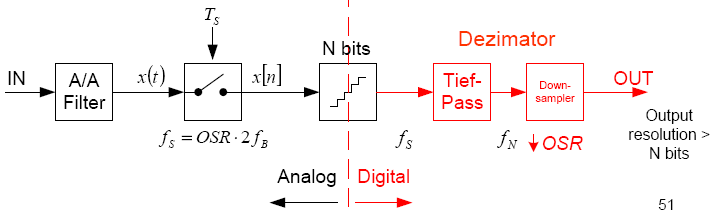
\includegraphics[width=1.0\textwidth]{images/Prinzipschema}
\end{minipage}
\hfill
\begin{minipage}{0.55\textwidth}
    \begin{compactitem}
        \item Rauschleistungsdichte im Basisband wird durch Überabtastung reduziert
        \item Quantisierer mit reduzierter Auflösung
        \item Dezimierung (Mittelwertbildung) erhöht Auflösung
        \item Einfacheres Anti-Aliasing Filter
    \end{compactitem}
\end{minipage}
\subsubsection{Prinzip der Sigma-Delta-Wandler}
\begin{minipage}{0.40\textwidth}
    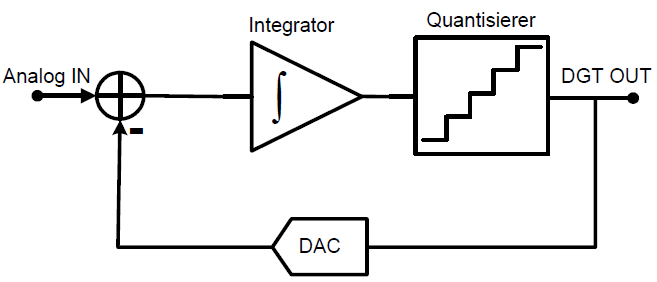
\includegraphics[width=1.0\textwidth]{images/Prinzipschema2}
\end{minipage}
\hfill
\begin{minipage}{0.55\textwidth}
    \begin{compactitem}
        \item Hohe Überabtastung $\rightarrow$ SNR-Gewinn von 3dB pro Oktave
        \item Durch negative Rückkoppelung wird Quantisierungsrauschen gefiltert und aus Signalfrequenzbereich entfernt $\rightarrow$ Noise shaping
        \item Integrator hat eine sehr grosse Verstärkung bei niedrigen Frequenzen $\rightarrow$ Hoher Loop-Gain
    \end{compactitem}
\end{minipage}
\subsubsection{Highlights der Sigma-Delta-Wandler}
\begin{minipage}{0.55\textwidth}
    \begin{compactitem}
        \item kleiner Analogteil, wenig Drift und kleine Temperaturabhängigkeit
        \item Monotone Funktion
        \item Linear
        \item Brauchen keine Sample-Hold
    \end{compactitem}
\end{minipage}
\hfill
\begin{minipage}{0.40\textwidth}
    \begin{compactitem}
        \item Einfache Anti-Aliasing-Filter
        \item Aufwändige Digitalfilter (können aber beispielsweise Netzbrumm filtern)
        \item Relativ billig
        \item Mit einem Bandpass-ADC sind auch relativ hohe Frequenzen verarbeitbar
    \end{compactitem}
\end{minipage}

\subsection{Aufbau von Sigma-Delta-Wandlern}
\begin{minipage}{0.55\textwidth}
    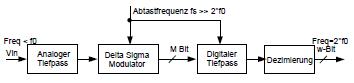
\includegraphics[width=1.0\textwidth]{images/AufbauSigmaDeltaWandler}
\end{minipage}
\hfill
\begin{minipage}{0.40\textwidth}
    \begin{compactitem}
        \item Analoger TP dient als Anti-Aliasing-Filter
        \item Der Modulator (wird sehr hoch getaktet) wandelt das analoge Signal in einen digitalen Datenstrom (mit Frequenz fs) um
        \item Datenstrom wird mit digitalem TP gefiltert und durch Dezimierung auf fNyquist reduziert 
    \end{compactitem}
\end{minipage}

\subsection{Sigma-Delta-Modulatoren}
\begin{minipage}{0.55\textwidth}
    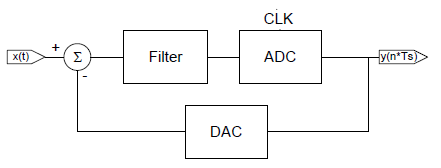
\includegraphics[width=1.0\textwidth]{images/AufbauSigmaDeltaModulator}
    \begin{compactitem}
        \item Vom Eingangssignal x(t) wird die Ausgangsspannung von einem DAC subtrahiert
        \item Dieses Differenz-Signal wird mit einem Filter (bei Modulatoren 1. Ordnung ein Integrator $\rightarrow$ sehr grosse Verstärkung bei niedrigen Frequenzen) gefiltert
    \end{compactitem}
\end{minipage}
\hfill
\begin{minipage}{0.40\textwidth}
    \begin{compactitem}
        \item Das Ausgangssignal des Filters wird mit einem ADC in eine zeitdiskrete Datenfolge umgewandelt. \item Der ADC-Wert steuert den DAC, dessen Ausgangsspannung von der Eingangsspannung subtrahiert wird
        \item ADC und DAC sind oft nur ein Bit breit, d.h. es sind Komparatoren resp. Umschalter zwischen zwei Spannungspegeln
    \end{compactitem}
\end{minipage}
\newpage
\subsection{Implementationen von Sigma-Delta-Modulatoren}
\textbf{Integrierender Wandler:}\\
\begin{minipage}{0.55\textwidth}
    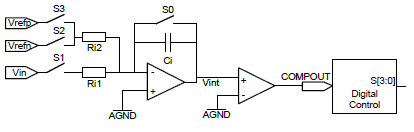
\includegraphics[width=1.0\textwidth]{images/IntegrierenderWandler}
\end{minipage}
\hfill
\begin{minipage}{0.40\textwidth}
    \begin{compactitem}
        \item Schaltung für Dual SlopeADC oder Modulator (je nach Schalter-Ansteuerung)
        \item Eingangsbereich Vin von Vrefn bis Vrefp (Ri1=Ri2)
        \item Vrefp und Vrefn symmetrisch um VAGND
    \end{compactitem}
\end{minipage}
\textbf{Charge Balancing Wandler:}\\
\begin{minipage}{0.55\textwidth}
    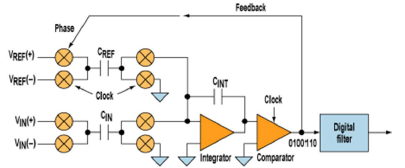
\includegraphics[width=1.0\textwidth]{images/ChargeBalancing}
\end{minipage}
\hfill
\begin{minipage}{0.40\textwidth}
     $\Delta Q_{Cint} = Cin \cdot Vin \pm Cref \cdot Vref$
    \\\\  $n = N \cdot \frac{Vin \cdot Cin + Vref \cdot Cref}{2 \cdot Vref \cdot Cref}$\\
    \begin{compactitem}
        \item Durch Zählen der "1" im Bitstream (n) kann Vin bestimmt werden: gleitender Mittelwert über N Takte
        \item Je grösser N, desto höher die Auflösung
        \item Kurzer Beobachtungszeitraum: Kleine Auflösung, dafür schnelle Reaktion auf Signalwechsel
        \item Langer Beobachtungszeitraum: Hohe Auflösung, dafür langsamere Reaktion auf Signalwechsel
    \end{compactitem}

\end{minipage}
\textbf{Modulator mit RC-Integrator:}\\
\begin{minipage}{0.55\textwidth}
    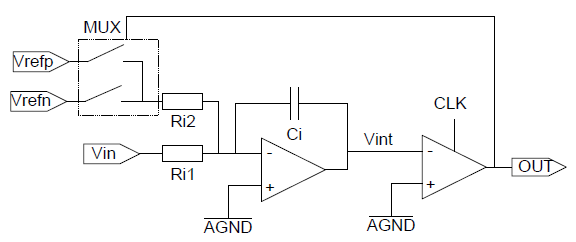
\includegraphics[width=1.0\textwidth]{images/SigmaDeltaDualSlope}
\end{minipage}
\hfill
\begin{minipage}{0.40\textwidth}
    \begin{compactitem}
        \item Komparator mit Flip-Flop für Synchronisierung mit CLK 
        \item Vrefp und VRrefn symmetrisch um AGND (+Vref, -Vref)
        \item AGND als virtueller Ground betrachtet (=0V)
        \item Ri1=Ri2, damit Bereich von Vin zw. Vrefp und Vrefn resp. +/-Vref
    \end{compactitem}
\end{minipage}
\begin{minipage}{0.45\textwidth}
    Vin=0V:\\
    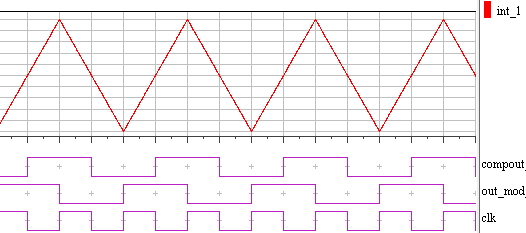
\includegraphics[width=1.0\textwidth]{images/Signal1}\\\\
    Vin=-0.5*Vref:\\
    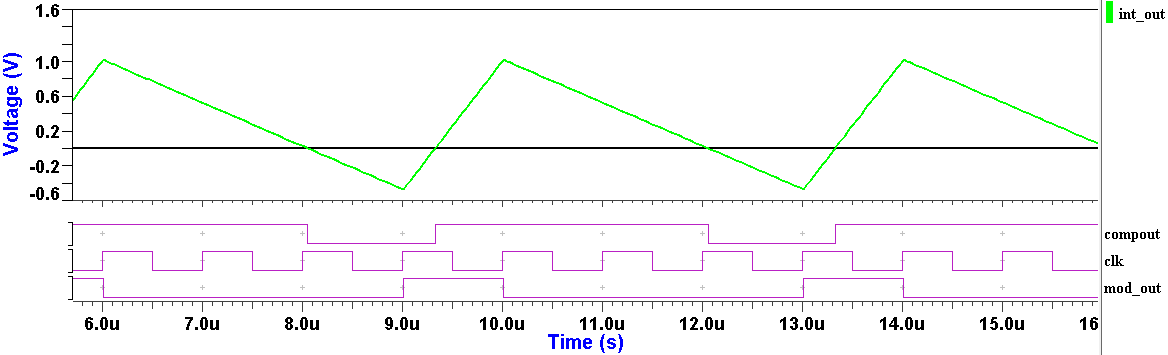
\includegraphics[width=1.0\textwidth]{images/Signal3}
\end{minipage}
\hfill
\begin{minipage}{0.45\textwidth}
    Vin=0.5*Vref:\\
    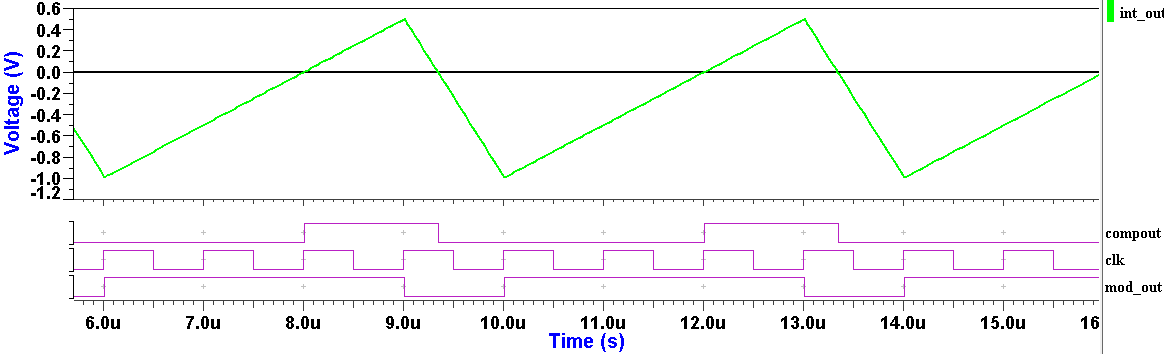
\includegraphics[width=1.0\textwidth]{images/Signal2}\\\\\\\\
    Vin=-7/8*Vref:\\
    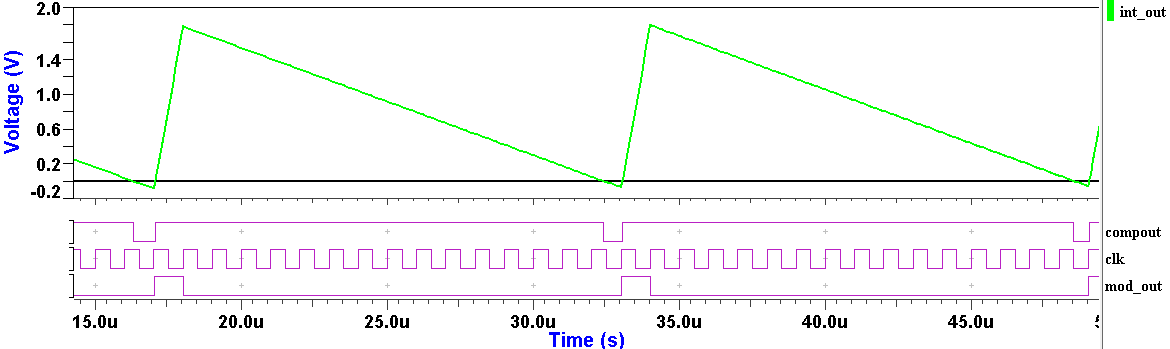
\includegraphics[width=1.0\textwidth]{images/Signal4}
\end{minipage}\\ \ \\ \ \\
\textbf{Pattern Noise:} Kurze repetitive Sequenzen erzeugen hohe Frequenzen, die vom Digitalfilter eliminiert werden. Längere repetitive Sequenzen können innerhalb des Signalfrequenzbandes liegen. Sie können nicht von niederfrequenten Eingangssignalen unterschieden werden und werden damit vom digitalen Filter nicht herausgefiltert.
Dieser Effekt heisst Pattern Noise und ist natürlich in vielen Applikationen inakzeptabel. In der Praxis werden deshalb nur selten Modulatoren 1. Ordnung verwendet. Bei Modulatoren höherer Ordnung entsteht kaum Pattern noise.

\subsection{Modellierung von Sigma-Delta Modulatoren}
\textbf{Laplace-Modell:}\\
\begin{minipage}{0.45\textwidth}
    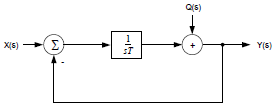
\includegraphics[width=1.0\textwidth]{images/SigmaDeltaLaplace}
\end{minipage}
\hfill
\begin{minipage}{0.45\textwidth}
   Ausgangssignal:\\ $Y(s)=[X(s)-Y(s)]\cdot \frac{1}{s \cdot T}$\\\\
   Signal-Übertragungsfunktion:\\ $H_{s}(s)=\frac{Y(s)}{X(s)}=\frac{1/(s \cdot T)}{1+1/(s\cdot T)} = \frac{1}{1+s\cdot T}$\\\\
   Rausch-Übertragungsfunktion:\\
   $H_{n}(s)=\frac{Y(s)}{Q(s)}=\frac{1}{1+1/(s\cdot T)} = \frac{s \cdot T}{1+ s \cdot T}$
\end{minipage}\\
Aus diesen beiden Übertragungsfunktionen lässt sich der Vorteil des Sigma-Delta Modulator erkennen. Für die Nutzsignale verhält er sich wie ein Tiefpass, für das Quantisierungsrauschen wie ein Hochpass. Mit anderen Worten: Die Nutzsignale werden nicht verändert, solange ihre Frequenzen nicht grösser sind als die Eckfrequenz des Tiefpasses. Die Sigma-Delta Schlaufe innerhalb des Modulators jedoch schiebt das Quantisierungsrauschen in höhere Frequenzbereiche. Dieses Verschieben wird als "Noise Shaping" bezeichnet.\\ \ \\
\textbf{Zeitdiskretes-Modell:}\\
\begin{minipage}{0.45\textwidth}
    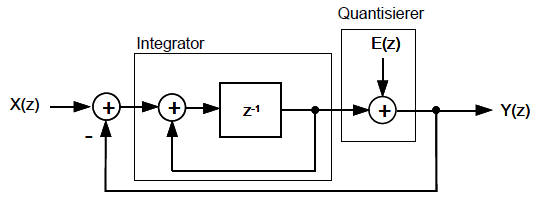
\includegraphics[width=1.0\textwidth]{images/SigmaDeltaZeitdiskretesModell}
\end{minipage}
\hfill
\begin{minipage}{0.45\textwidth}
    Differenzengleichung:\\ $y(n) = x(n-1)+[e(n)-e(n-1)]$\\\\
    Z-Transformation:\\ $Y(z)=z^{-1}\cdot X(z)+E(z)\cdot (1-z^{-1})$\\\\
    Fehlerübertragungsfunktion:\\
    $H_{E1}(z) = E(z) \cdot (1-z^{-1})$\\\\
    Rauschdichte:\\ $N(f)=\sqrt{\frac{2}{fs}}\cdot \frac{q}{12} \cdot 2 \cdot sin(\frac{2 \cdot \pi \cdot f}{fs})$\\\\
    Effektivwert der Rausch-Spannung:\\
    $n0=\frac{q}{\sqrt{12}}\cdot \frac{\pi ^2}{\sqrt{3}}\cdot (\frac{2 \cdot f0}{fs})^\frac{3}{2}$
\end{minipage}


%\subsection{Multibit-Modulatoren}
%Es gibt 2 Möglichkeiten, eine vorgegebene Auflösung zu erreichen: Die Änderung der Überabtastungsrate und der Auflösung des ADC. Für Wandler mit hohen Auflösungsanforderungen (hohes SNR) können Multibit- Modulatoren eingesetzt werden, wenn die Abtastfrequenz nicht erhöht werden kann.

\subsection{Sigma-Delta Modulator 2.Ordnung}
Beim Modulator 2.Ordnung werden ein zweiter Integrator und ein zweiter Summationsknoten addiert.
\begin{minipage}{0.45\textwidth}
    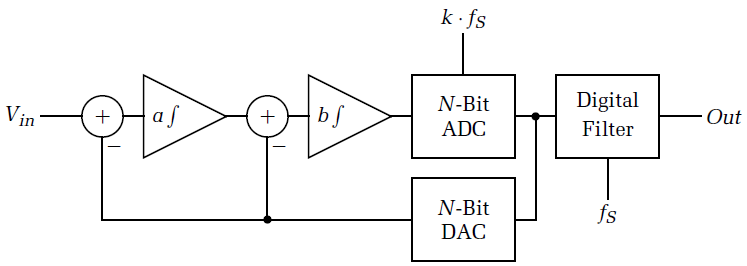
\includegraphics[width=1.0\textwidth]{images/SigmaDelta2Ordnung}
    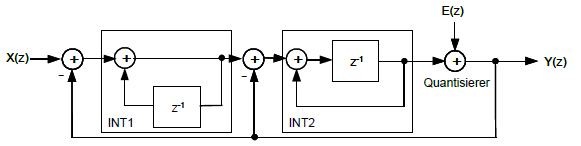
\includegraphics[width=1.0\textwidth]{images/SigmaDeltaZeitdiskretesModell2}
\end{minipage}
\hfill
\begin{minipage}{0.45\textwidth}
    Differenzengleichung:\\
    $y(n) = x(n-1) + e(n) -2e(n-1) + e(n-2)$\\\\
    Z-Transformation:\\ $Y(z)= z^{-1} \cdot X(z) + E(z) \cdot (1-2\cdot z^{-1} + z^{-2}) = z^{-1} \cdot X(z) + E(z) \cdot (1-z^{-1})^2$\\\\
    Fehlerübertragungsfunktion:\\
    $H_{E2}(z) = E(z) \cdot (1-z^{-1})^2$\\\\
    Effektivwert des Quantisierungsrauschens:\\
    $n0=\frac{q}{\sqrt{12}}\cdot \frac{\pi ^2}{\sqrt{5}}\cdot (\frac{2 \cdot f0}{fs})^\frac{5}{2}$
    
\end{minipage}
\subsection{Modulatoren höherer Ordnung}
\begin{compactitem}
    \item Modulatoren mit Ordnungen \textgreater 2 können instabil werden
    \item Effekt der spektralen Verschiebung des Quantisierungsrauschens wird weiter verstärkt
    \item Noise Shaping funktioniert nicht nur bei tiefen Frequenzen und Tiefpass-Filtern sondern auch mit Bandpass-Filtern $\rightarrow$ Bandpass Sigma-Delta-Wandler
\end{compactitem}

\subsection{Dynamikgewinn durch Sigma-Delta Modulatoren}
Werden die einzelnen Fehlerfunktionen untersucht, so stellt man fest, dass mit jeder Erhöhung der Ordnung eines Sigma-Delta Modulators die Hochpass Funktion kaskadiert wird. Mit jeder Erhöhung der Ordnung steigt der Signalrauschabstand um 6dB pro Oktave an, was dem Anstieg eines Integrators entspricht: $SNR = 10 \cdot log_{10} (\frac{3}{2} \cdot \frac{2M+1}{\pi^{2M}}\cdot OSR^{2M+1})$\ \ \ \ \
$OSR=fs/2f0$ \ \ \ \ \ M = Modulatorordnung\\ 
\textbf{Bei einer Verdoppelung der Abtastrate wird der Dynamikbereich um 9dB oder 1.5 Bit erhöt!}

